\documentclass[oneside, final, 14pt]{extreport} %односторонняя печать, чистовик, размер текста
\usepackage[utf8]{inputenc} %кодировка
\usepackage[english,russian]{babel} %языки
\usepackage{vmargin} %пакет для регулировки отступов
\setmarginsrb{2cm}{1.5cm}{1cm}{1.5cm}{0pt}{0mm}{0pt}{13mm} %Регулируем отступы
\setpapersize{A4}
\usepackage{indentfirst} %Чтобы первый абзац начинался с отступа
\sloppy %Чтобы текст ни в коем случае не залезал на поля


%код выше не трогаем. Это шапка
\linespread{1.5} % Полуторный интервал


\usepackage{chngcntr} %пакет, чтобы пофиксить нумерацию
\counterwithout{section}{chapter} %отключает учет номера главы при нумерации секций, что позволяет секциям 
%начинаться с 1 вместо 0. 
%\renewcommand{\thesection}{\arabic{section}.0} %Задаём нумерацию в формате number.0

%графика
\usepackage{graphicx}%Вставка картинок правильная
\usepackage{float}%"Плавающие" картинки
\usepackage{wrapfig}%Обтекание фигур (таблиц, картинок и прочего)





%для кода
\usepackage{listings}
\usepackage[T2A,T1]{fontenc}
\usepackage[utf8]{inputenc}

\usepackage{listings}




%Чтобы в списке литературы было написано "Источники", а не Литература
\addto\captionsrussian{\renewcommand{\bibname}{Источники}}


\title{Справочная информация по системе Linux}
\author{Алексей Полухин}
\date{2023}


\begin{document}

\begin{titlepage}
    \maketitle
\end{titlepage}

\begin{figure}[ht]
    \centering
    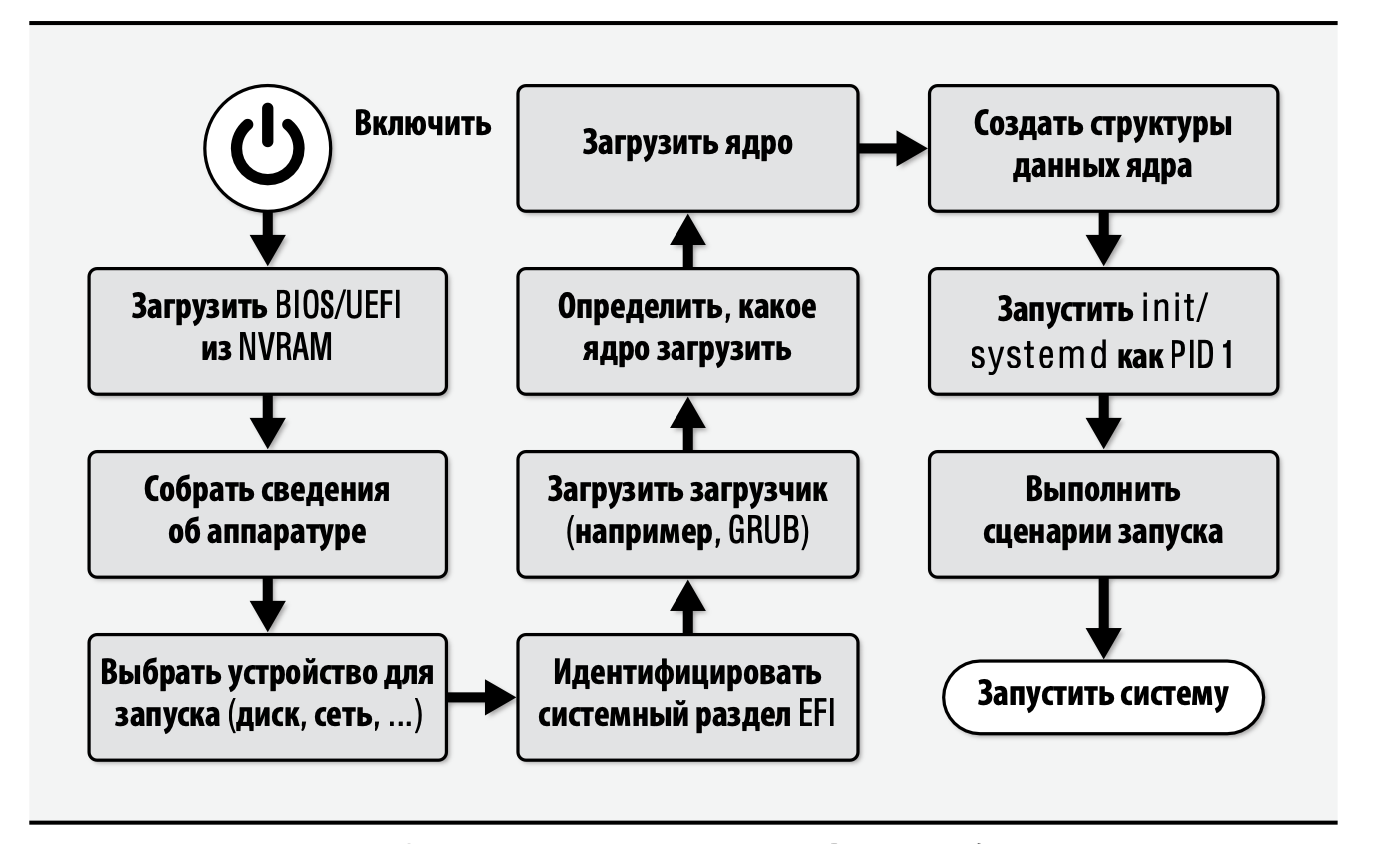
\includegraphics[width=0.9\textwidth]{1.png}
    \caption{Процессы загрузки Linux и Unix}
    \label{fig:1}
\end{figure}

\section{Справочная информация. Полезные сведения}


\textbf{Демон в Linux} – \textit{фоновый процесс}. Программа на уровне пользователя

\textit{Киби-, меби-, гиби-} байты

\textit{репозиторий} --- место, где хранятся и \textbf{поддерживаются} какие-то данные
Примеры репозиториев: \textit{App Store, Google Play}

\section{Операционные системы}

\subsection{Ядро ОС}

\textit{Ядро ОС} – центральная часть ОС, обеспечивающая приложениям 
координированный доступ к ресурсам комьютера Рис.~\ref{fig:3}. 
В современных ОС приложение не может напрямую обратиться 
к ресурсам комьютера, поэтому приложения обращаются к \textbf{ядру}.

\begin{figure}[ht]
    \centering
    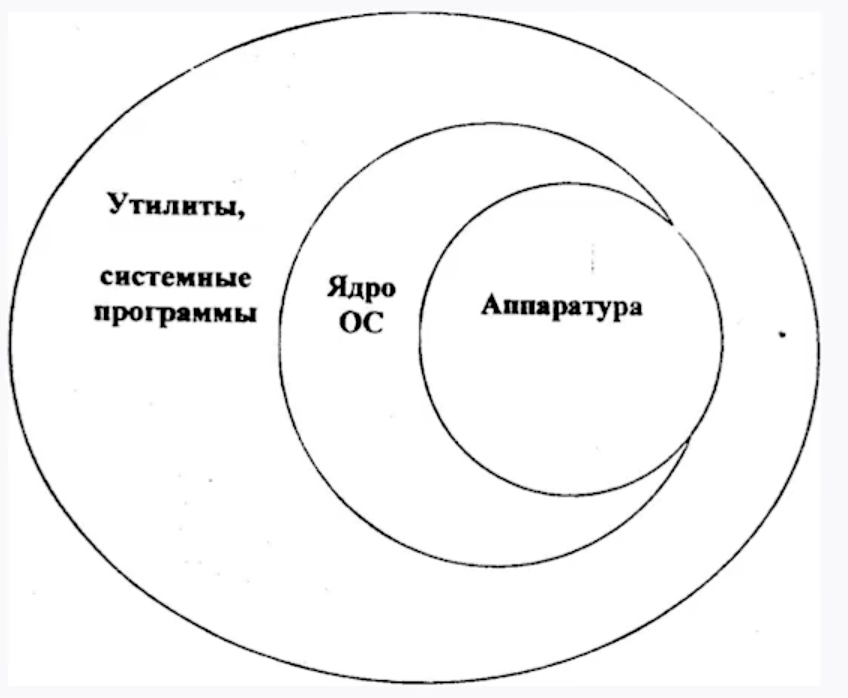
\includegraphics[width=0.5\textwidth]{3.png}
    \caption{Ядро ОС}
    \label{fig:3}
\end{figure}

\textit{Архитектура ядра операционной системы} --- это структура и дизайн основной части операционной системы, которая обеспечивает основные функции управления ресурсами компьютера, планирование выполнения задач, обработку прерываний и обеспечивает взаимодействие между аппаратными устройствами и пользовательскими процессами.

В ОС, основанных на ядре, приложения имеют собственные независимые окружения. То есть
свои участки памяти, своё процессорное время, свой доступ к устройствам 
ввода и вывода.


Современные ОС имеют пространство ядра (где идёт работа с оборудованием)
и пространство пользователя.

\textit{\textbf{Архитектуры ядер}}
\begin{itemize}
    \item Монолитное ядро (самое быстрое) --- Linux
    \item Микроядро (самое отказоустойчивое)
    \item Гибридное ядро --- Windows
\end{itemize}

Ближе к оборудованию --- быстрее, ближе к пространству пользователя --- стабильнее.
(Интересная аналогия: Python, C++, assembler)

Создание ОС с ядром возможно, когда на аппаратном уровне появляются
кольца защиты. (методы разграничения ресурсов компьютера)

\textit{Кольца защиты} --- аппаратная реализация механизма
разграничения ресурсов компьютера 


Интерпретатор команд --- это обычное приложение. В Linux
они бывают разные: \textit{shell, bash, ksh, csh, psh \ldots} Он не 
является частью ядра ОС.

Для Linux не существует расширений файлов, они сделаны 
исключительно для удобства пользователя и для программ, которые 
взаимодействуют с этими файлами

Всё в Unix/Linux --- это файл, просто поток байт

\vspace{\baselineskip} %добавление интервала пустой строчки

\subsection{\textit{UNIX}}

\textit{\textbf{Философия UNX}}
\begin{enumerate}
    \item \textbf{Пишите программы, которые делают что-то одно, но хорошо}
    \item Пишите программы, кототрые работают вместе 
    \item Пишите программы, кототрые поддерживали бы текстовые потоки, так как это универсальный интерфейс
\end{enumerate}

\vspace{\baselineskip} %добавление интервала пустой строчки
 
\textit{POSIX} --- набор стандартов, описывающих 
инетерфейсы между операционной системой и 
прикладной прогаммой (в \textit{UNIX}). (Средство общения 
с ядром ОС). Обеспечивает 
совместимость UNIX-подобных ОС.

Когда разработчики создают программы, используя стандарт POSIX, эти программы могут работать на разных операционных системах без необходимости изменять их код. Это облегчает перенос программного обеспечения с одной системы на другую, так как программы, сделанные в соответствии с POSIX, будут использовать одни и те же команды и функции, доступные во всех системах, поддерживающих этот стандарт.

\textit{POSIX} описывает работу в пространстве пользователя. (видимо, 
именно из-за этого команды в терминалах MacOS, Unix и Linux совпадают)

Команды вроде ls (список файлов и директорий) и pwd (текущая рабочая директория) являются стандартными командами, определенными в стандарте POSIX.

POSIX определяет интерфейс и поведение для командной оболочки и других системных команд в операционных системах, таких как UNIX, Linux, macOS и другие, чтобы обеспечить переносимость программ между различными системами.

Сейчас UNIX используется в серверах и мейнфреймах

\textit{Мейнфрейм (Mainframe)} --- это тип большого и мощного компьютера, который обычно используется в корпоративных средах для обработки больших объемов данных и критически важных бизнес-приложений.
(Например, используется в центрах усправления (космическими) полётами, в банках, на биржах --- в отраслях, где
важна каждая \textit{наносекунда}). (Используется в критически важных задачах, где
важна скорость и бесперебойность)

На всех суперкопьютерах установлен Linux, потому что они решают сложные математические
задачи, если они вдруг остановятся, ничего критического не произойдёт.






\subsection{Структура каталогов в Linux}

См. Рис.~\ref{fig:4}

Основные каталоги
\begin{itemize}
    \item / --- root
    \item /bin --- Необходимые утилиты, необходимые при работе всем пользователям (и в однопользовательском режиме)
    \item /boot --- загрузочные файлы (файлы загрузчика, ядро, initrd, System.tap)
    \item /dev --- основные файлы устройств
    \item \textbf{/etc} --- общесистемные конфигурационные файлы (настройки) (настройки ОС и служб ОС)
    \item /home --- домашние каталоги пользователей (их персональные настройки и данные)
    \item /lib --- Основные библиотеки, необходимые для работы программ из /bin и /sbin 
    \item /media --- Каталог, где производится монтирование сменных носителей (USB, CD-ROM)
    \item /mnt --- каталог содержит временно монтирование файловые системы 
    \item /opt --- Дополнительные программное обеспечение 
    \item \textbf{/proc} --- каталог, которые содержит информацию о всех процессах в нашей ОС
    \item /root --- домашний каталог пользователя \textit{root}
    \item /run --- информация о системе с момента её загрузки (что запущено и чем это работает)
    \item /sbin --- основные системные исполняемые файлы (основыне программы для настройки и администрирования сисетмы, \textit{init, ifcondif, iptables})
    \item /srv --- данные для серисов, представляемых системой (\textit{www} или \textit{ftp})
    \item \textbf{/sys} --- содержит информацию об устройствах, драйверах и некоторых свойствах ядра
    \item /tmp --- временные файлы
    \item /usr --- Большинство пользовательских приложений и утилит (используемых в многопользовательском режиме)
    \item /var --- изменяемые файлы. (файлы регистрации, временные почтовые файлы, файлы спулеров)
    \item /var/log --- логи
    \item /home/username --- домашний каталог пользователя 
\end{itemize}

\subsection{Установка ПО в Linux}

\textit{Установка ПО в Linux/Unix --- это просто переписывание бинарных файлов}

\textit{пакет} --- скомпилированный бинарный файл и перечень зависимостей

\begin{enumerate}
    \item Из исходных кодов (файлы на языке С) --- \textbf{плохой способ}
     \begin{itemize}
        \item Можно модифицировать и устанавливать без прав администртора
        \item Поиск зависимостей очень долгий (как и сам процесс компиляции)
        \item Нет контроля ПО. (что, какой версии, куда, когда и кто установил --- нет возможности узнать)
        \item Правильнее будет скопиллировать, собрать пакет и пакет установить с помощью пакетоного менеджера (будет вестись запись установленного ПО и версий)
     \end{itemize}
    \item Из пакетов 
    \begin{itemize}
        \item Сразу видны зависимости
        \item Не тратится время на компилляцию 
        \item Просто распаковка архива и копирование файлов в нужное место ОС (если есть все  зависимсти)
        \item Есть контроль версий ПО 
        \item Нужны права администратора 
        \item Пакеты создаются под определённый дистрибутив Linux 
    \end{itemize}
    \item Из репозитория --- \textbf{лучший способ}
    \begin{itemize}
        \item Сразу виден перечень зависимостей 
        \item Есть контроль версий ПО 
        \item Как правило, все зависимости устанавливаются автоматически из репозитория
        \item При установке пакетный менеджер сообщит, что нужно и сколько места это займёт
        \item Репозиторий может быть локально или где-то на серверах
    \end{itemize}
\end{enumerate}

\begin{figure}[ht]
    \centering
    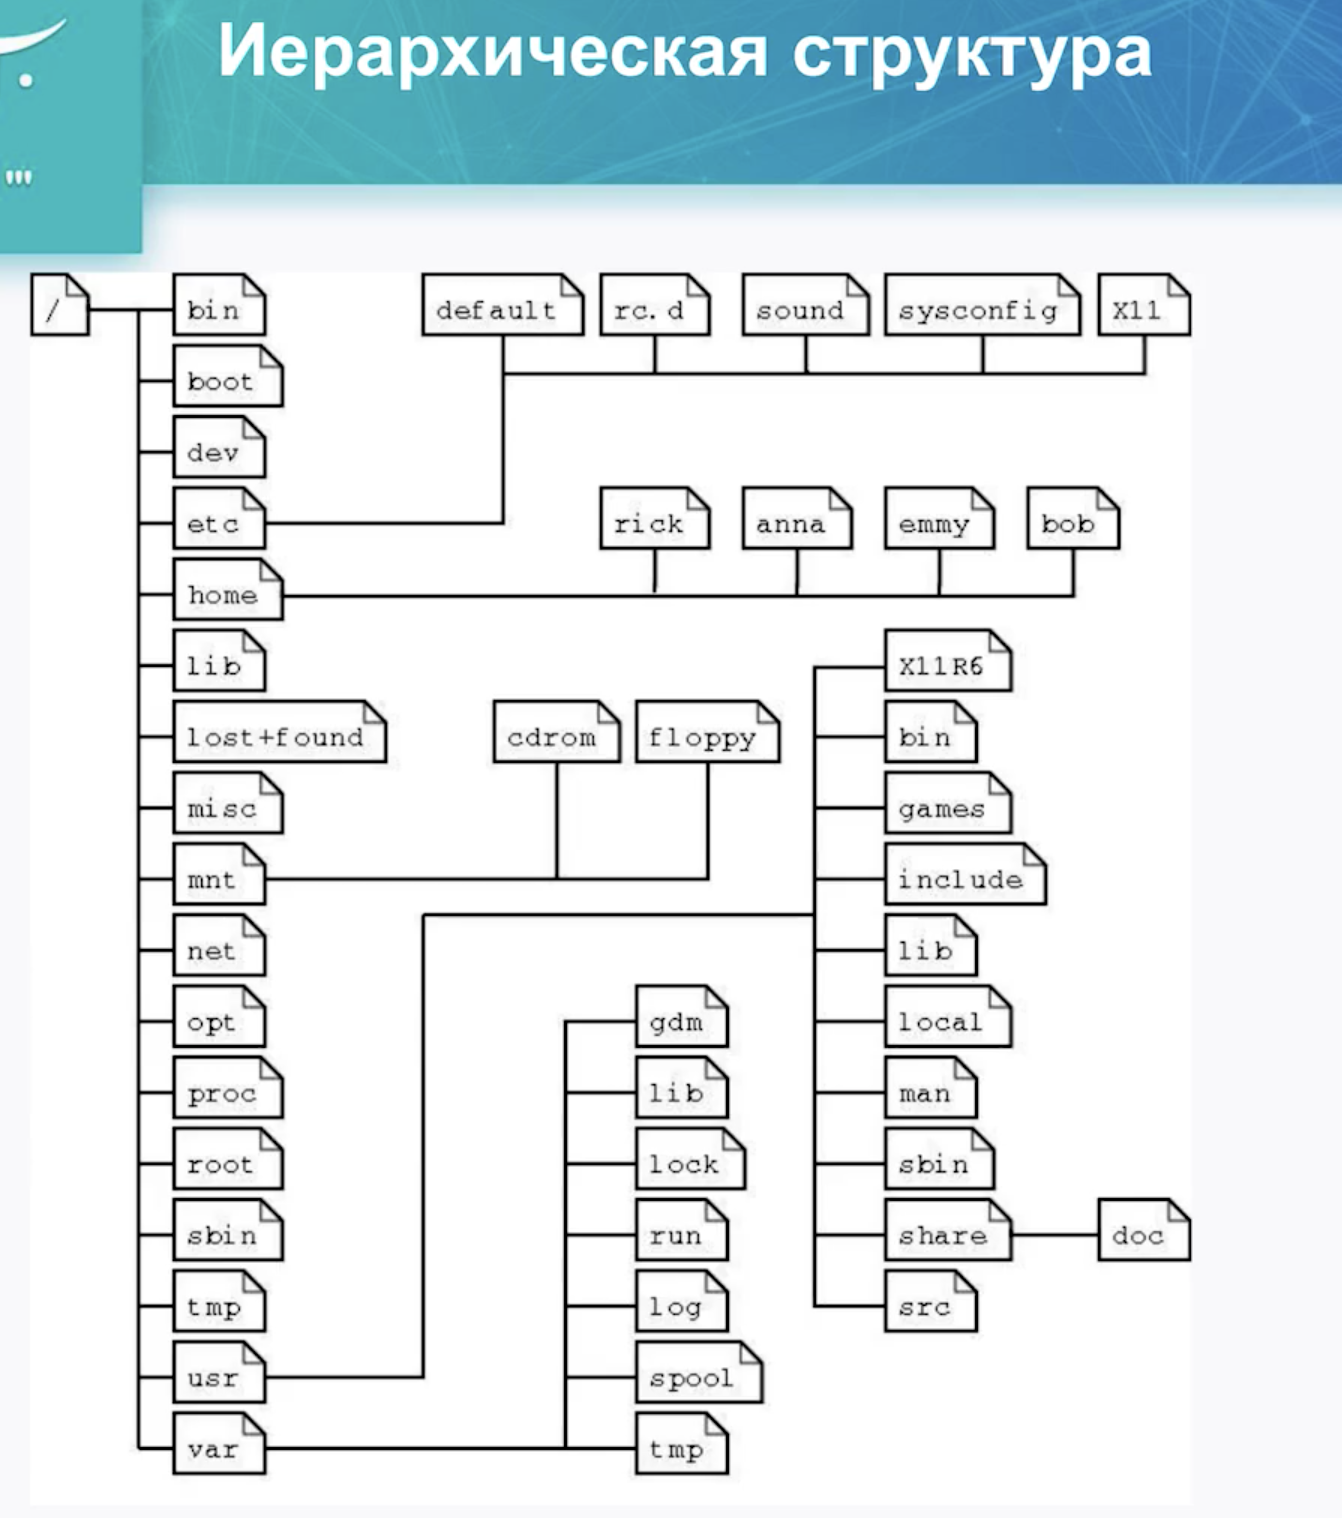
\includegraphics[width=0.6\textwidth]{4.png}
    \caption{Структура каталогов в Linux}
    \label{fig:4}
\end{figure}

\subsection{Создание Linux}
Linus Torvalds в 1991 создал \textit{\textbf{ядро}} операционной системы Linux.
Ядро --- часть ОС, которая отвечает за взаимодействие с оборудованием и предоставляет
определённый интерфейс (в данном случае \textit{POSIX})
Пользователи и администраторы не работают с самим ядром, они работают в пространстве пользователя

У Richard M. Stallman было готово окружение GNU, но не было ядра. 

Проекты объединились и образовалась ОС GNU/Linx. 
OC GNU/Linux --- это ядро и набор программ. 

Официальная версия ядра vanilla kernel \textit{www.kernel.org/}

\vspace{\baselineskip}
\textit{\textbf{Различия дистрибутив}}
\begin{itemize}
    \item Разные версии ядра
    \item Разная структура каталогов
    \item Разные менеджеры пакетов
\end{itemize}

\section{Полезные bash-команды}

Формат:

\textbf{команда} \textit{ключи} \textbf{\textit{аргументы}}

\vspace{\baselineskip}

\$ man -k word –– \textit{ищёт в документации ключевое слово word}

\$ uname --- выводит информацию о версии ядра

\$ date --- выводит текущую дату и время

\$ ls -l --- более подробный ls

(Если в первой колонке вывода \$ \textit{ls -l} стоит \textbf{-}, то это файл. А если \textbf{d} --- то директория)

\$ ls -la (или -l -a) --- посмотреть скрытые файлы (имя начинаются с .~)

\$ ls -la .. --- содержимое родительского каталога

\$ \textit{comand} \--\--help --- справочная информация

\$ touch \textit{existing\_file} --- изменить время создания файла

\$ mkdir -p dir1/dir2/dir3 --- рекурсивное создание директорий

Двойное нажатие TAB выдаст спсиок возможных дополнений. Кроме того, если дополнение единственное, 
будет дополено автоматически

\$ cd --- переводит в домашную директорию пользователя (аналог cd \textasciitilde).

Конструкция \$ cd alex эквивалентна \$ cd ./alex

\vspace{\baselineskip}
\textbf{Маски для файлов (<<Регулярные выражения>>)}

* --- любой набор любых символов

? --- один любой символ

\$ rm *2 --- (всё, что оканчивается на 2)

\$ rm file* --- (всё, что начинается с file)

\$ rm *.pdf --- (все pdf файлы)

\$ rm garbadge.*













\subsection{Пример сборки кода из исходников}


%код
%\begin{lstlisting}
%here we can write some code
%\end{lstlisting}
    

\$ git clone https:/github.com/the-tcpdump-qroup/tcpdump.qit

\$ cd tcpdump

\$ ./confiqure

\$ make

\$ sudo make install

\subsection{Зависимости}

\begin{table}[h]
    \centering
    \begin{tabular}{|c|c|}
    \hline
    Wants & Модули, которые должны быть активированы одновременно,\\ 
    & если это возможно, но не обязательно \\
    \hline
    Requires & Строгие зависимости; отказ от каких-либо предварительных условий \\ 
    &прекращает работу этой службы \\
    \hline
    Requisite & Аналогично \textit{Requires}, но модуль должен быть активным \\
    \hline
    BindsTo & Аналогично \textit{Requires}, но модуль должен быть связан еще более тесно \\
    \hline
    PartOf & Аналогично Requires, но влияет только на запуск и остановку \\
    \hline
    Сonf1iсts & Отрицательные зависимости; не может взаимодействовать \\ &
    с этими единицами \\
    \hline
    \end{tabular}
    \caption{Явные зависимости}
\end{table}

\section{Полезные слайды}

\begin{figure}[t]
    \centering
    %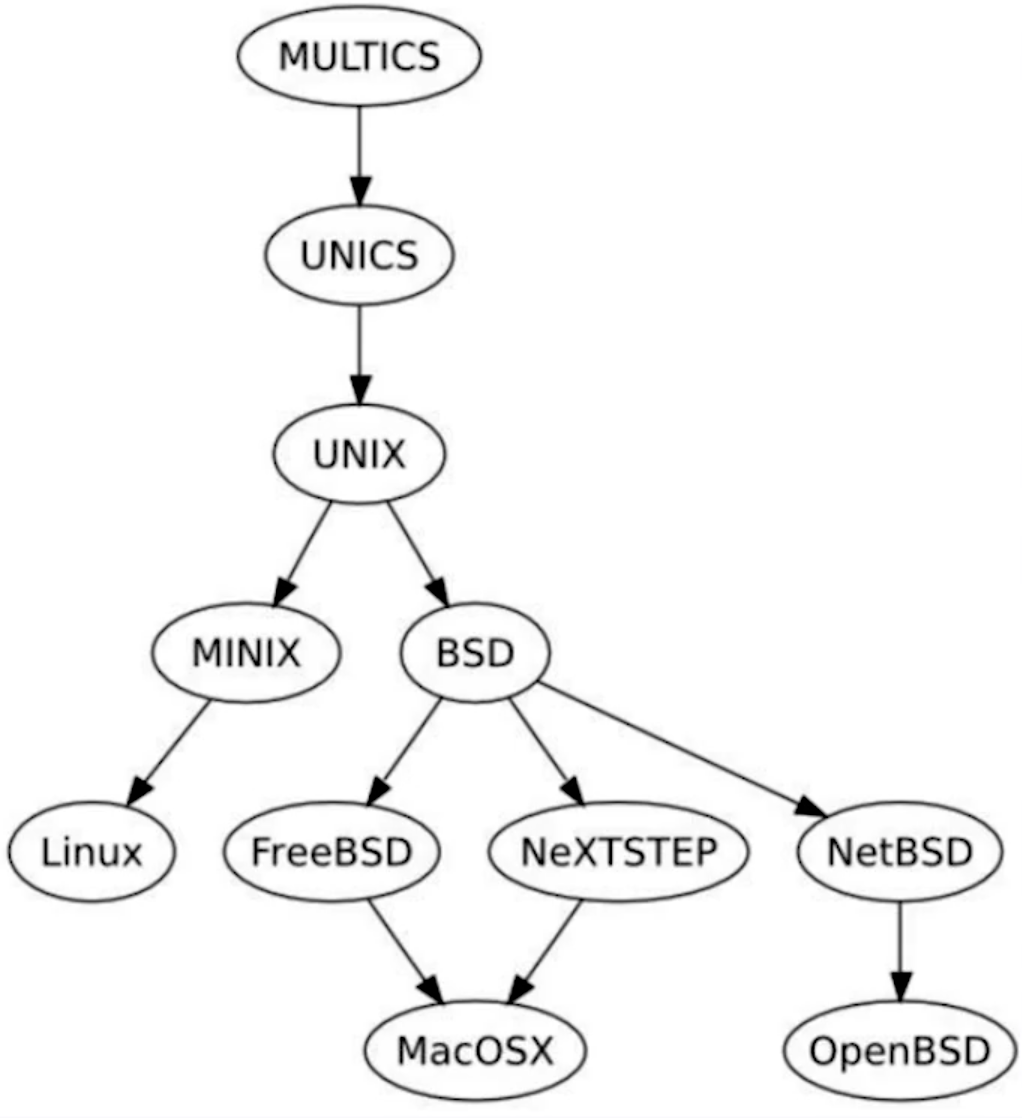
\includegraphics[width=0.2\textwidth]{2.png}
    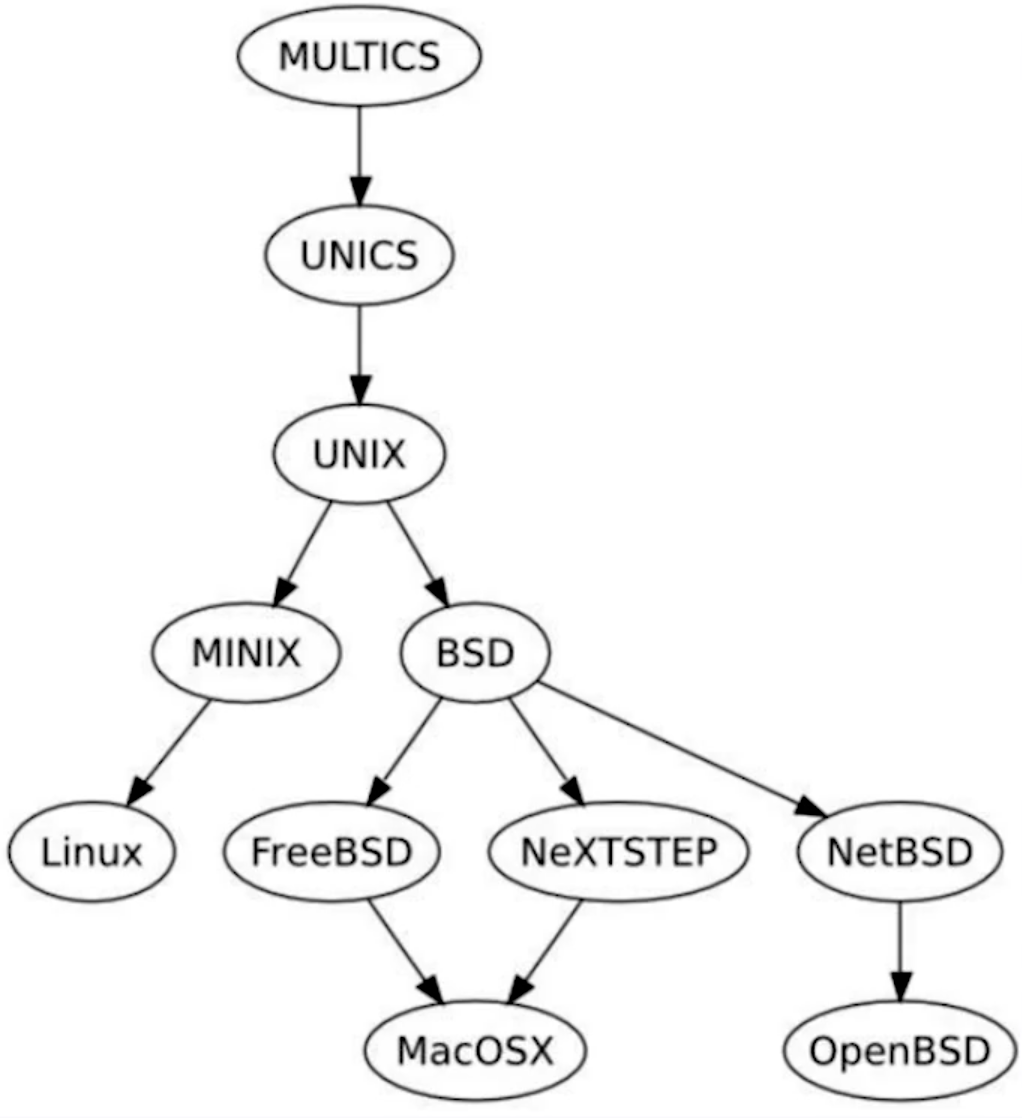
\includegraphics[height=0.3\textheight]{2.png}
    \caption{Развитие операционных систем}
    \label{fig:2}

\end{figure}

\end{document}